\chapter{Pemanfaatan Bandwidth: Multiplexing dan Spreading}

Telah kita ketahui bersama bahwa dalam komunikasi data diharapkan agar kecepatan data dapat dicapai setinggi-tingginya sedangkan kecepatan pengiriman sinyal dapat dicapai serendah-rendahnya. Kecepatan data tinggi dalam proses transmisi berarti bahwa sejumlah besar data dapat dikirimkan dalam satu satuan waktu. Karena itu semakin tinggi data rate berarti semakin besar jumlah data yang dapat dikirimkan dalam satu satuan waktu. Sedangkan kecepatan pengiriman sinyal diharapkan menjadi rendah karena berkaitan dengan bandwidth dari suatu saluran.

Pada kenyataanya kita hanya memiliki saluran dengan bandwidth terbatas, sedangkan seringkali kita menggunakan beberapa aplikasi dengan saluran komunikasi yang sama. Oleh karena itu, penggunaan bandwidth perlu dilakukan secara bijak. Aktivitas penggunaan bandwidth telah, dan akan menjadi, salah satu tantangan utama pada setiap komunikasi elektronik. Terkadang kita membutuhkan untuk menggabungkan beberapa channel (dengan bandwidth rendah) untuk mendapatkan channel dengan bandwidth yang lebih besar. Terkadang kita perlu untuk memperlebar bandwidth untuk mendapat suatu tujuan seperti privacy dan antijamming. Pada bab ini kita akan mempelajari dua teori dasar tentang penggunaan Bandwidth yaitu \textit{multiplexing} dan \textit{spreading}. Pada \textit{multiplexing} tujuan kita adalah efisiensi; kita menggabungkan beberapa channel menjadi jadi satu. Sedangakan pada \textit{spreading}, tujuan kita adalah \textit{privacy} dan \textit{antijamming} sehingga kita melakukan pelebaran untuk memasukkan \textit{redundancy}, dimana diperlukan untuk mendapatkan tujuan tersebut. 


\section{Multiplexing}
Perlu diketahui bahwa jika bandwidth dari sebuah saluran yang menghubungkan dua buah devais adalah lebih besar dari pada bandwidth yang dibutuhan devais, maka saluran (\textit{link}) tersebut dapat di \textit{sharing}. \textit{Multiplexing} merupakan seperangkat teknik yang memungkinkan transmisi secara simultan dari beberapa sinyal melalui sebuah \textit{data link}. Seiring meningkatnya penggunaan data dan telekomunikasi, semakin tinggi pula lalu lintas data yang terjadi. Untuk mengakomodasi peningkatan ini dapat dilakukan penambahan \textit{link} setiap saat \textit{channel} baru dibutuhkan; atau kita dapat memasang \textit{link} dengan bandwidth yang lebih lebar dan menggunakan setiap \textit{channel} untuk membawa beberapa sinyal. Saat ini, teknologi dengan media \textit{high-bandwidth} seperti fiber optik dan satelit gelombang mikro memiliki \textit{bandwidth} yang jauh lebih besar dibandingkan \textit{bandwidth} yang dibutuhkan untuk melakukan transmisi sinyal. Jika \textit{bandwidth} sebuah \textit{link} lebih besar dari pada \textit{bandwidth} yang dibutuhan oleh perangkat yang tehubung ke \textit{link} tersebut, maka \textit{bandwidth} sia-sia. Oleh karena itu, diperlukan sebuah sistem yang akan memaksimalkan penggunaan semua \textit{resource}; \textit{bandwidth} adalah salah satu dari \textit{resource} yang paling berharga dalam komunikasi data.

Pada sistem multipleks, n jalur (\textit{line}) berbagi \textit{bandwidth} dari satu \textit{link}. Dapat dilihat pada gambar~\ref{fig6:1}, ilustrasi format dasar dari sistem multipleks. Jalur di bagian kiri mengarahkan aliran transmisinya langsung ke \textit{multiplexer} (MUX), yang menggabungkannya menjadi satu aliran (\textit{many-to-one}). Di sisi penerima, aliran tersebut dimasukkan ke dalam demultiplexer (DEMUX), pada DEMUX aliran dipisahkan kembali ke transmisi komponennya (one-to-many) dan mengarahkannya ke jalur yang sesuai. Pada gambar~\ref{fig6:1}, kata link mengacu pada jalur fisik. Kata saluran (channel) mengacu pada bagian dari link yang membawa transmisi antara sepasang garis tertentu. Satu link dapat memiliki banyak (n) saluran

\begin{figure}[htbp]
  \centering
  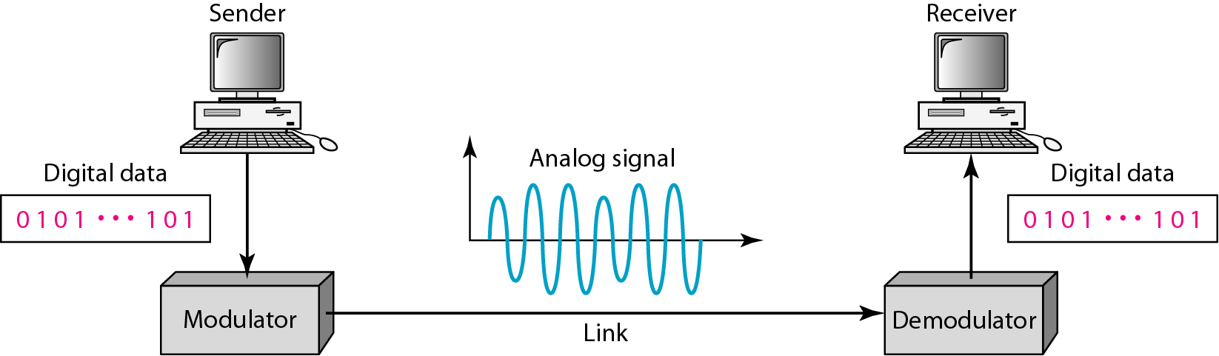
\includegraphics[width=0.9\columnwidth]{bab6/Picture1}
  \caption{Pembagian 1 link ke n-channel}
  \label{fig6:1}
\end{figure}

Terdapat tiga teknik dasar pada multipleksing, yaitu:
\begin{itemize}
  \item frequency-division multiplexing
  \item wavelength-division multiplexing
  \item time-division multiplexing
\end{itemize}
untuk teknik frequency-division multiplexing dan wavelength-division multiplexing didesain untuk sinyal analog, sedangkan teknik time-division multiplexing didesain untuk sinyal digital.

\subsection{Frequency-Division Multiplexing}
Frequency-division multiplexing (FDM) merupakan teknik analog yang dapat diterapkan ketika bandwidth sebuah link (dalam Hertz) lebih besar dari pada bandwidth dari gabungan seluruh sinyal yang ditransmisikan. Dengan kata lain, FDM adalah teknik multiplexing analog yang menggabungkan sinyal analog. Pada FDM, sinyal dibangkitkan oleh setiap perangkat pengirim memodulasi frekuensi carrier yang berbeda. Sinyal termodulasi ini kemudian digabungkan menjadi satu sinyal komposit yang dapat ditransmisikan oleh link. Carrier frequencies are separated by sufficient bandwidth to accommodate the modulated signal. These bandwidth ranges are the channels through which the various signals travel. Channels can be separated by strips of unused bandwidth-guard bands-to prevent signals from overlapping. In addition, carrier frequencies must not interfere with the original data frequencies.

\begin{figure}[htbp]
  \centering
  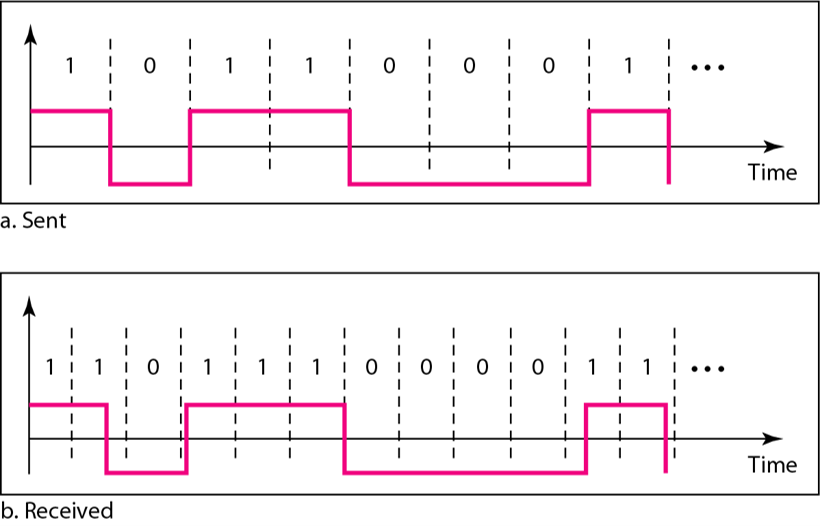
\includegraphics[width=0.9\columnwidth]{bab6/Picture3}
  \caption{Ilustrasi Frequency-division multiplexing}
  \label{fig6:2}
\end{figure}

Telah kita ketahui FDM sebagai teknik multiplexing untuk sinyal analog; namun, ini tidak berarti bahwa FDM tidak dapat digunakan untuk menggabungkan sumber yang mengirimkan sinyal digital. Untuk melakukan penggabungan sinyal digital menggunakan FDM, sebuah sinyal digital dapat dikonversikan menjadi sinyal analog terlebih dahulu sebelum FDM diterapkan.

\subsection*{Proses Multipleksing}
Ilustrasi konseptual dari proses multipleksing dapat dilihat pada


\begin{figure}[htbp]
  \centering
  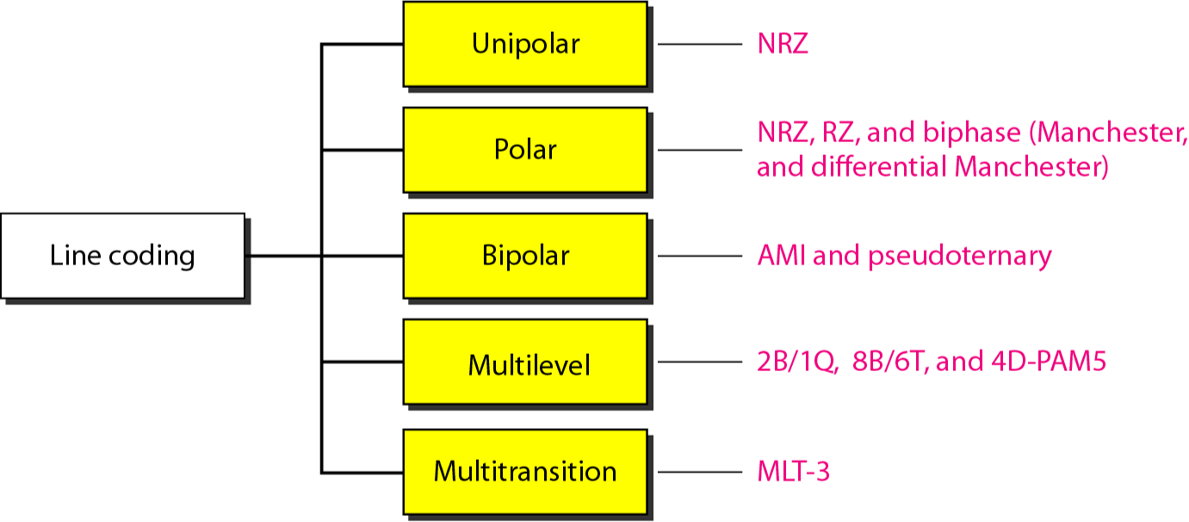
\includegraphics[width=0.9\columnwidth]{bab6/Picture4}
  \caption{Proses Frequency-division multiplexing}
  \label{fig6:3}
\end{figure}

\subsection*{Proses Demultipleksing}
The demultiplexer uses a series of filters to decompose the multiplexed signal into its constituent component signals. The individual signals are then passed to a demodulator that separates them from their carriers and passes them to the output lines.

\begin{figure}[htbp]
  \centering
  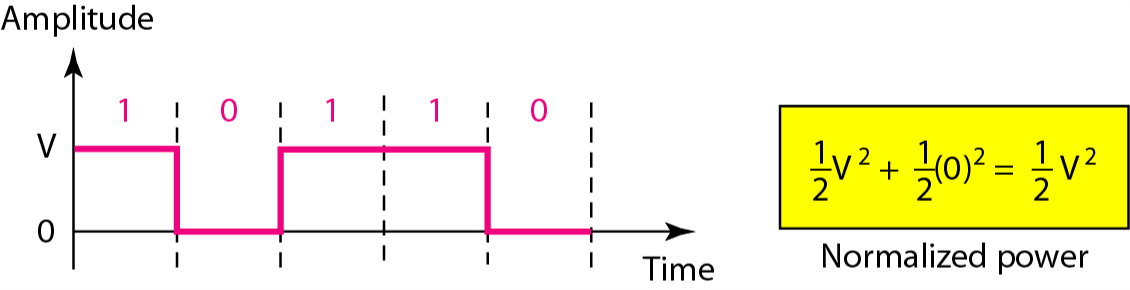
\includegraphics[width=0.9\columnwidth]{bab6/Picture5}
  \caption{Ilustrasi demultipleksing pada FDM}
  \label{fig6:4}
\end{figure}


\begin{example}
  Assume that a voice channel occupies a bandwidth of 4 kHz. We need to combine three voice channels into a link with a bandwidth of 12 kHz, from 20 to 32 kHz. Show the configuration, using the frequency domain. Assume there are no guard bands.
  \label{example6:1}
\end{example}

\begin{solution}
  We shift (modulate) each of the three voice channels to a different bandwidth, as shown in Figure 6.6. We use the 20- to 24-kHz bandwidth for the first channel, the 24- to 28-kHz bandwidth for the second channel, and the 28- to 32-kHz bandwidth for the third one. Then we combine them as shown in Figure~\ref{fig6:5}. At the receiver, each channel receives the entire signal, using a filter to separate out its own signal. The first channel uses a filter that passes frequencies between 20 and 24 kHz and filters out (discards) any other frequencies. The second channel uses a filter that passes frequencies between 24 and 28 kHz, and the third channel uses a filter that passes frequencies between 28 and 32 kHz. Each channel then shifts the frequency to start from zero
\end{solution}

\begin{figure}[htbp]
  \centering
  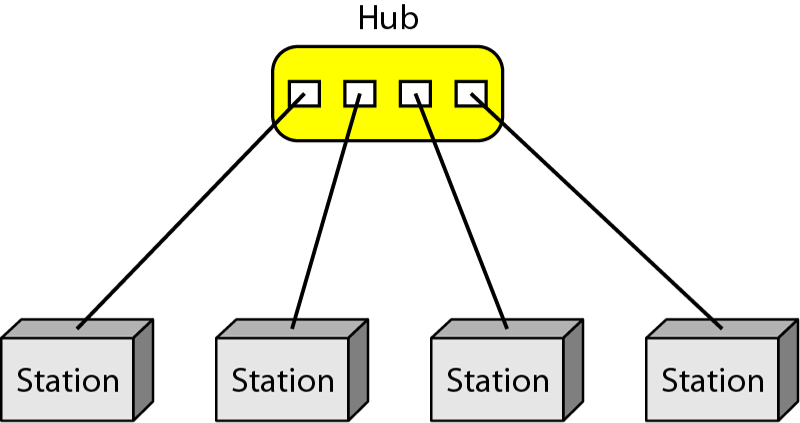
\includegraphics[width=0.9\columnwidth]{bab6/Picture6}
  \caption{Ilustrasi untuk contoh~\ref{example6:1}}
  \label{fig6:5}
\end{figure}

\begin{example}
  Five channels, each with a lOa-kHz bandwidth, are to be multiplexed together. What is the minimum bandwidth of the link if there is a need for a guard band of 10kHz between the channels to prevent interference?
  \label{example6:2}
\end{example}

\begin{solution}
  For five channels, we need at least four guard bands. This means that the required bandwidth is at least 5 x 100 + 4 x 10 =540 kHz, as shown in Figure~\ref{fig6:6}
\end{solution}

\begin{figure}[htbp]
  \centering
  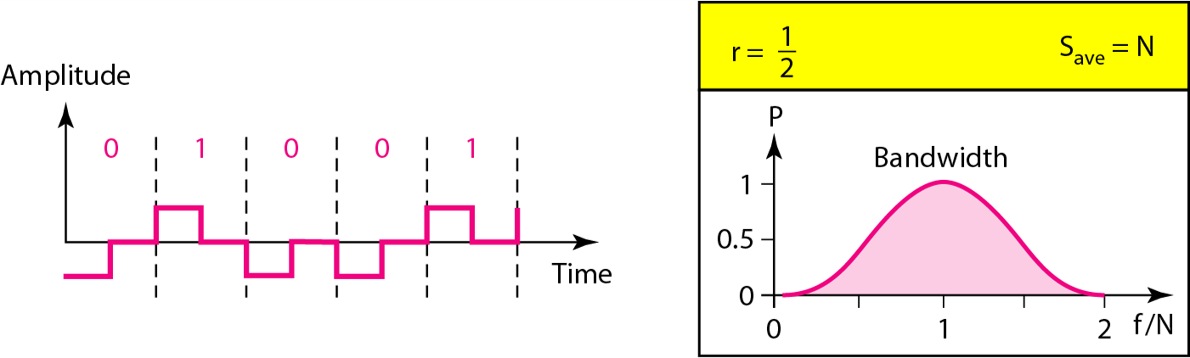
\includegraphics[width=0.9\columnwidth]{bab6/Picture7}
  \caption{Ilustrasi untuk contoh~\ref{example6:2}}
  \label{fig6:6}
\end{figure}

\begin{example}
  Four data channels (digital), each transmitting at 1 Mbps, use a satellite channel of 1 MHz. Design an appropriate configuration, using FDM.
  \label{example6:3}
\end{example}

\begin{solution}
  The satellite channel is analog. We divide it into four channels, each channel having a 2S0-kHz bandwidth. Each digital channel of I Mbps is modulated such that each 4 bits is modulated to 1 Hz. One solution is 16-QAM modulation. Figure~\ref{fig6:7} shows one possible configuration
\end{solution}

\begin{figure}[htbp]
  \centering
  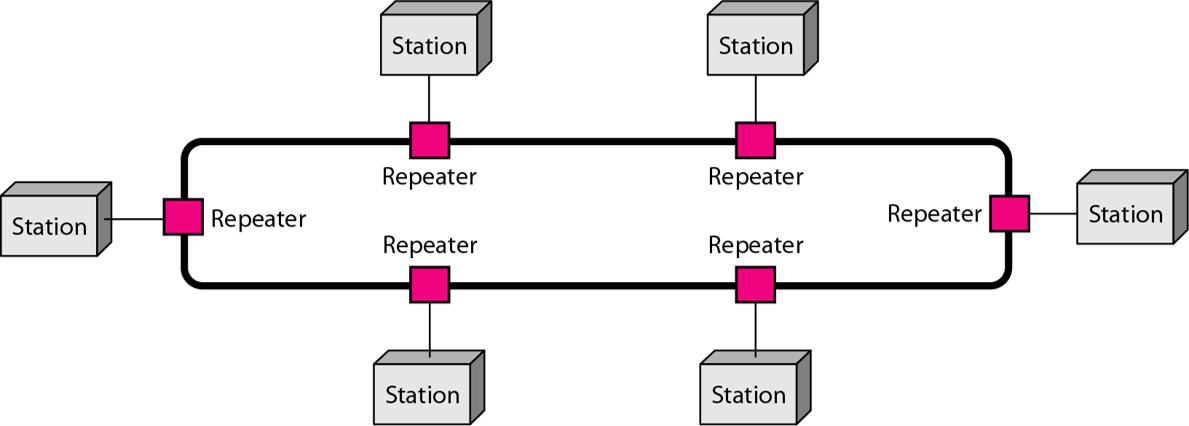
\includegraphics[width=0.9\columnwidth]{bab6/Picture8}
  \caption{Ilustrasi untuk contoh~\ref{example6:3}}
  \label{fig6:7}
\end{figure}

\subsection*{Analog Carrier System}
To maximize the efficiency of their infrastructure, telephone companies have traditionally multiplexed signals from lower-bandwidth lines onto higher-bandwidth lines. In this way, many switched or leased lines can be combined into fewer but bigger channels. For analog lines, FDM is used.

One of these hierarchical systems used by AT\&T is made up of groups, supergroups, master groups, and jumbo groups (see Figure~\ref{fig6:8})

\begin{figure}[htbp]
  \centering
  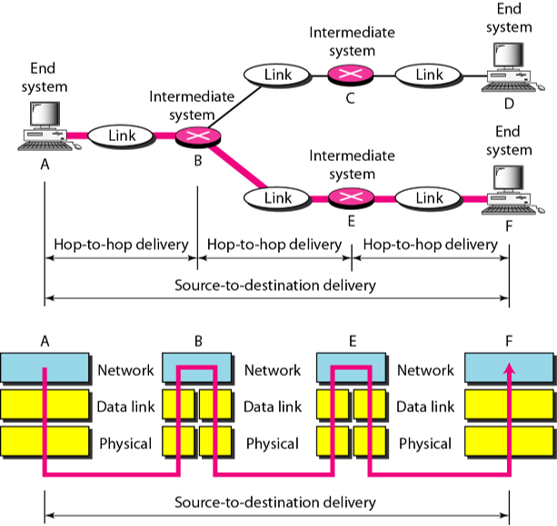
\includegraphics[width=0.9\columnwidth]{bab6/Picture9}
  \caption{Ilustrasi untuk contoh~\ref{example6:3}}
  \label{fig6:8}
\end{figure}

In this analog hierarchy, 12 voice channels are multiplexed onto a higher-bandwidth line to create a group. A group has 48 kHz of bandwidth and supports 12 voice channels.

At the next level, up to five groups can be multiplexed to create a composite signal called a supergroup. A supergroup has a bandwidth of 240 kHz and supports up to 60 voice channels. Supergroups can be made up of either five groups or 60 independent voice channels.

At the next level, 10 supergroups are multiplexed to create a master group. A master group must have 2.40 MHz of bandwidth, but the need for guard bands between the supergroups increases the necessary bandwidth to 2.52 MHz. Master groups support up to 600 voice channels.

Finally, six master groups can be combined into a jumbo group. A jumbo group must have 15.12 MHz (6 x 2.52 MHz) but is augmented to 16.984 MHz to allow for guard bands between the master groups.

\subsection*{Aplikasi lain dari FDM}
A very common application of FDM is AM and FM radio broadcasting. Radio uses the air as the transmission medium. A special band from 530 to 1700 kHz is assigned to AM radio. All radio stations need to share this band. As discussed in Chapter 5, each AM station needs 10kHz of bandwidth. Each station uses a different carrier frequency, which means it is shifting its signal and multiplexing. The signal that goes to the air is a combination of signals. A receiver receives all these signals, but filters (by tuning) only the one which is desired. Without multiplexing, only one AM station could broadcast to the common link, the air. However, we need to know that there is physical multiplexer or demultiplexer here.

The situation is similar in FM broadcasting. However, FM has a wider band of 88 to 108 MHz because each station needs a bandwidth of 200 kHz. Another common use of FDM is in television broadcasting. Each TV channel has its own bandwidth of 6 MHz.

The first generation of cellular telephones (still in operation) also uses FDM. Each user is assigned two 30-kHz channels, one for sending voice and the other for receiving. The voice signal, which has a bandwidth of 3 kHz (from 300 to 3300 Hz), is modulated by using FM. Remember that an FM signal has a bandwidth 10 times that of the modulating signal, which means each channel has 30 kHz (10 x 3) of bandwidth. Therefore, each user is given, by the base station, a 60-kHz bandwidth in a range available at the time ofthe call.

\vspace{12pt}

\begin{example}
  The Advanced Mobile Phone System (AMPS) uses two bands. The first band of 824 to 849 MHz is used for sending, and 869 to 894 MHz is used for receiving. Each user has a bandwidth of 30 kHz in each direction. The 3-kHz voice is modulated using FM, creating 30 kHz of modulated signal. How many people can use their cellular phones simultaneously?
  \label{example6:4}
\end{example}

\begin{solution}
  Each band is 25 MHz. If we divide 25 MHz by 30 kHz, we get 833.33. In reality, the band is divided into 832 channels. Of these, 42 channels are used for control, which means only 790 channels are available for cellular phone users.
\end{solution}

\subsection*{Implementasi FDM}
FDM can be implemented very easily. In many cases, such as radio and television broadcasting, there is no need for a physical multiplexer or demultiplexer. As long as the stations agree to send their broadcasts to the air using different carrier frequencies, multiplexing is achieved. In other cases, such as the cellular telephone system, a base station needs to assign a carrier frequency to the telephone user. There is not enough bandwidth in a cell to permanently assign a bandwidth range to every telephone user. When a user hangs up, her or his bandwidth is assigned to another caller.

\subsection{Wavelength-Division Multiplexing}
Wavelength-division multiplexing (WDM) adalah teknik multiplexing analog untuk menggabungkan sinyal optik. WDM dirancang untuk menggunakan kemampuan kecepatan data tinggi (\textit{high-data-rate}) dari kabel serat optik. The optical fiber data rate is higher than the data rate of metallic transmission cable. Using a fiber-optic cable for one single line wastes the available bandwidth. Multiplexing allows us to combine several lines into one.

WDM is conceptually the same as FDM, except that the multiplexing and demultiplexing involve optical signals transmitted through fiber-optic channels. The idea is the same: We are combining different signals of different frequencies. The difference is that the frequencies are very high

Figure~\ref{fig6:9} gives a conceptual view of a WDM multiplexer and demultiplexer. Very narrow bands of light from different sources are combined to make a wider band of light. At the receiver, the signals are separated by the demultiplexer.

\begin{figure}[htbp]
  \centering
  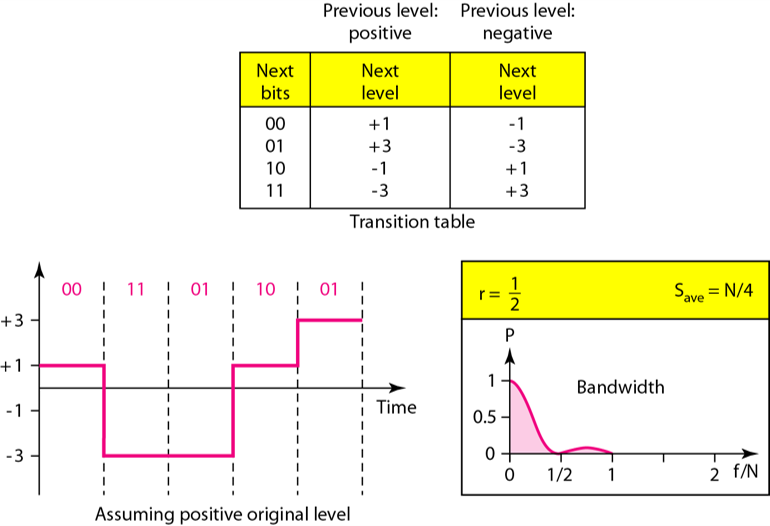
\includegraphics[width=0.9\columnwidth]{bab6/Picture10}
  \caption{Wavelength-division multiplexing}
  \label{fig6:9}
\end{figure}

Although WDM technology is very complex, the basic idea is very simple (ilustrasi dapat dilihat pada gambar~\ref{fig6:10}). We want to combine multiple light sources into one single light at the multiplexer and do the reverse at the demultiplexer. The combining and splitting of light sources are easily handled by a prism. Recall from basic physics that a prism bends a beam of light based on the angle of incidence and the frequency. Using this technique, a multiplexer can be made to combine several input beams of light, each containing a narrow band of frequencies, into one output beam of a wider band of frequencies. A demultiplexer can also be made to reverse the process.

\begin{figure}[htbp]
  \centering
  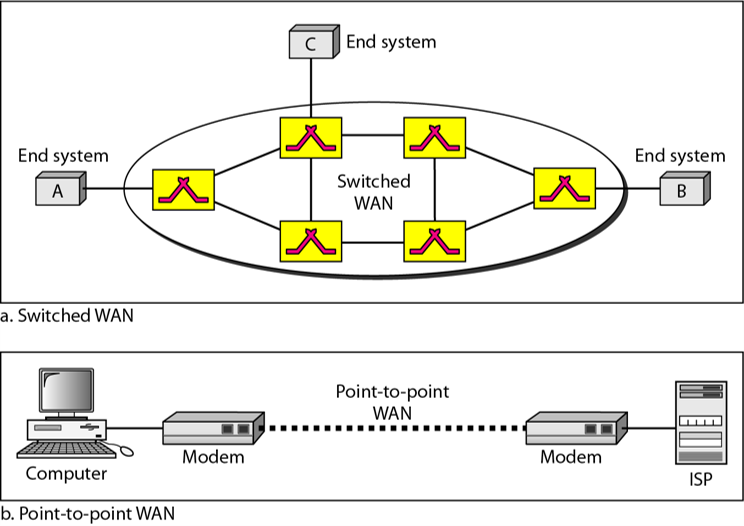
\includegraphics[width=0.9\columnwidth]{bab6/Picture11}
  \caption{Prisms in wavelength-division multiplexing and demultiplexing}
  \label{fig6:10}
\end{figure}

One application of WDM is the SONET network in which multiple optical fiber lines are multiplexed and demultiplexed. SONET (Synchronous Optical Network) adalah standar untuk menghubungkan sistem transmisi serat optik yang hanya dijual di Amerika Utara. SONET diusulkan oleh Bellcore pada pertengahan 1980-an dan sekarang menjadi standar ANSI. SONET mendefinisikan standar antarmuka pada lapisan fisik model tujuh lapisan Open Systems Interconnection (OSI). Standar tersebut mendefinisikan hierarki kecepatan antarmuka yang memungkinkan aliran data pada kecepatan yang berbeda untuk dimultipleks.

A new method, called dense WDM (DWDM), can multiplex a very large number of channels by spacing channels very close to one another. It achieves even greater efficiency.

\subsection{Synchronous Time-Division Multiplexing}
Time-division multiplexing (TDM) is a digital process that allows several connections to share the high bandwidth of a linle Instead of sharing a portion of the bandwidth as in FDM, time is shared. Each connection occupies a portion of time in the link. Figure~\ref{fig6:11} gives a conceptual view of TDM. Note that the same link is used as in FDM; here, however, the link is shown sectioned by time rather than by frequency. In the figure, portions of signals 1,2,3, and 4 occupy the link sequentially.

\begin{figure}[htbp]
  \centering
  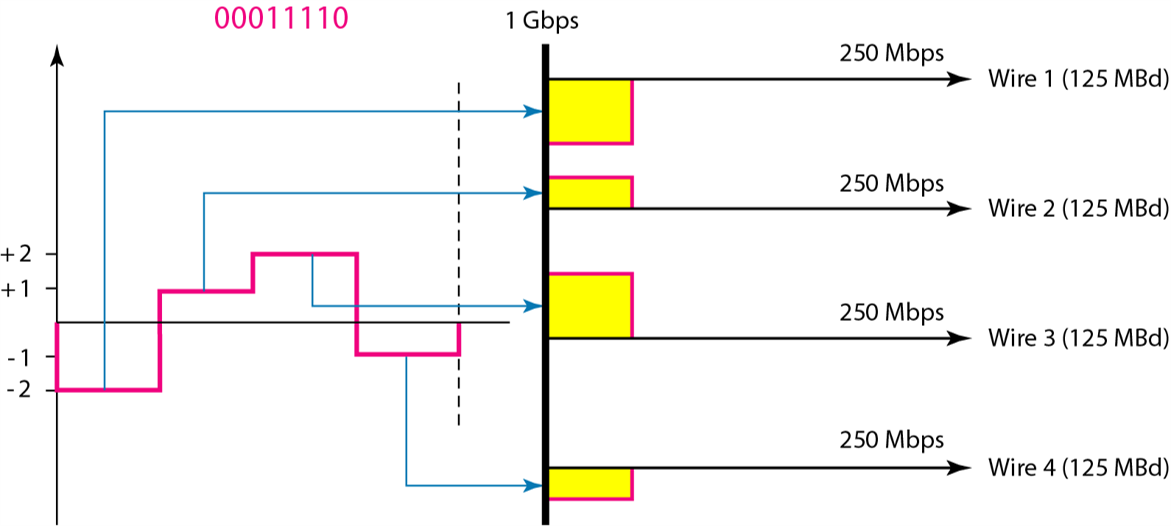
\includegraphics[width=0.9\columnwidth]{bab6/Picture12}
  \caption{Time-division multiplexing}
  \label{fig6:11}
\end{figure}

Note that in Figure~\ref{fig6:11} we are concerned with only multiplexing, not switching. This means that all the data in a message from source 1 always go to one specific destination, be it 1, 2, 3, or 4. The delivery is fixed and unvarying, unlike switching

We also need to remember that TDM is, in principle, a digital multiplexing technique for combining several low-rate channels into one high-rate one. Digital data from different sources are combined into one timeshared link. However, this does not mean that the sources cannot produce analog data; analog data can be sampled, changed to digital data, and then multiplexed by using TDM.

We can divide TDM into two different schemes: synchronous and statistical. We first discuss synchronous TDM and then show how statistical TDM differs. In synchronous TDM, each input connection has an allotment in the output even if it is not sending data.

\subsection*{Time Slots and Frames}
In synchronous TDM, the data flow of each input connection is divided into units, where each input occupies one input time slot. A unit can be 1 bit, one character, or one block of data. Each input unit becomes one output unit and occupies one output time slot. However, the duration of an output time slot is n times shorter than the duration of an input time slot. If an input time slot is T s, the output time slot is Tin s, where n is the number of connections. In other words, a unit in the output connection has a shorter duration; it travels faster. Figure~\ref{fig6:12} shows an example of synchronous TDM where n is 3.

\begin{figure}[htbp]
  \centering
  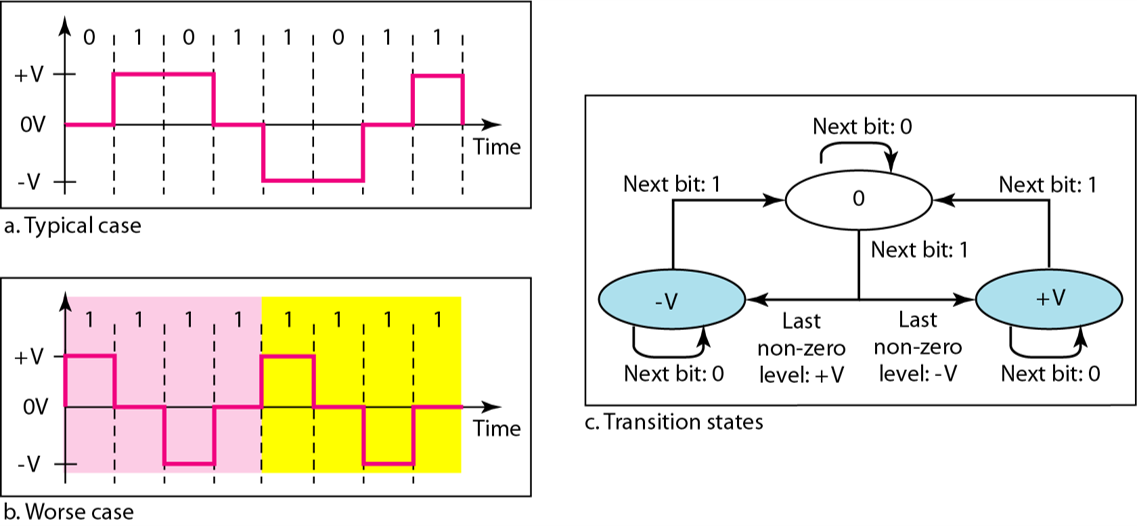
\includegraphics[width=0.9\columnwidth]{bab6/Picture13}
  \caption{Synchronous time-division multiplexing}
  \label{fig6:12}
\end{figure}

In synchronous TDM, a round of data units from each input connection is collected into a frame (we will see the reason for this shortly). If we have n connections, a frame is divided into n time slots and one slot is allocated for each unit, one for each input line. If the duration of the input unit is T, the duration of each slot is Tin and the duration of each frame is T (unless a frame carries some other information, as we will see shortly).

The data rate of the output link must be n times the data rate of a connection to guarantee the flow of data. In Figure 6.13, the data rate of the link is 3 times the data rate of a connection; likewise, the duration of a unit on a connection is 3 times that of the time slot (duration of a unit on the link). In the figure we represent the data prior to multiplexing as 3 times the size of the data after multiplexing. This is just to convey the idea that each unit is 3 times longer in duration before multiplexing than after.

In synchronous TDM, the data rate of the link is n times faster, and the unit duration is n times shorter.

Time slots are grouped into frames. A frame consists of one complete cycle of time slots, with one slot dedicated to each sending device. In a system with n input lines, each frame has n slots, with each slot allocated to carrying data from a specific input line.

\vspace{12pt}

\begin{example}
  In Figure~\ref{fig6:12}, the data rate for each input connection is 3 kbps. If 1 bit at a time is multiplexed (a unit is 1 bit), what is the duration of (a) each input slot, (b) each output slot, and (c) each frame?
  \label{example6:5}
\end{example}

\begin{solution}
  We can answer the questions as follows:
  \begin{itemize}
    \item[a.] The data rate of each input connection is 1 kbps. This means that the bit duration is 111000 s or 1 ms. The duration of the input time slot is 1 ms (same as bit duration).
    \item[b.] The duration of each output time slot is one-third of the input time slot. This means that the duration of the output time slot is 1/3 ms.
    \item[c.] Each frame carries three output time slots. So the duration of a frame is 3 $\times$ 113 ms, or 1 ms. The duration of a frame is the same as the duration of an input unit.
  \end{itemize}
\end{solution}

\vspace{12pt}

\begin{example}
  Figure~\ref{fig6:13} shows synchronous TOM with a data stream for each input and one data stream for the output. The unit of data is 1 bit. Find (a) the input bit duration, (b) the output bit duration, (c) the output bit rate, and (d) the output frame rate
  \label{example6:6}
\end{example}

\begin{figure}[htbp]
  \centering
  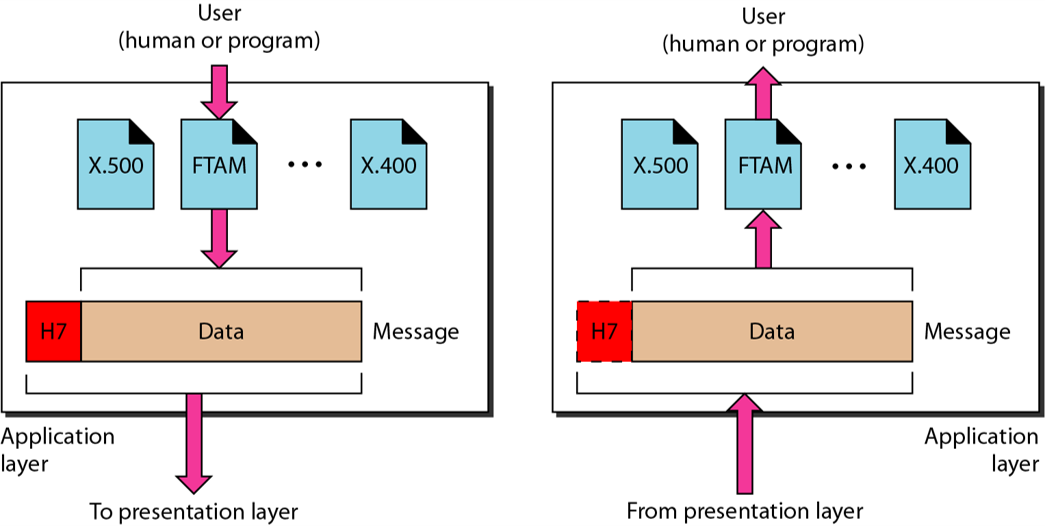
\includegraphics[width=0.9\columnwidth]{bab6/Picture14}
  \caption{Ilustrasi untuk contoh~\ref{example6:6}}
  \label{fig6:13}
\end{figure}

\begin{solution}
  We can answer the questions as follows:
  \begin{itemize}
    \item[a.] The input bit duration is the inverse of the bit rate: 1/1 Mbps = 1 $\mu$s.
    \item[b.] The output bit duration is one-fourth of the input bit duration, or 1/4 $\mu$s.
    \item[c.] The output bit rate is the inverse of the output bit duration or 1/4 $\mu$s, or 4 Mbps. This can also be deduced from the fact that the output rate is 4 times as fast as any input rate; so the output rate =4 x 1 Mbps =4 Mbps
    \item[d.] The frame rate is always the same as any input rate. So the frame rate is 1,000,000 frames per second. Because we are sending 4 bits in each frame, we can verify the result of the previous question by multiplying the frame rate by the number of bits per frame
  \end{itemize}
\end{solution}

\vspace{12pt}

\begin{example}
  Four l-kbps connections are multiplexed together. A unit is I bit. Find (a) the duration of I bit before multiplexing, (b) the transmission rate of the link, (c) the duration of a time slot, and (d) the duration of a frame
  \label{example6:7}
\end{example}

\begin{solution}
  We can answer the questions as follows: 
  \begin{itemize}
    \item[a.] The duration of 1 bit before multiplexing is 1/1 kbps, or 0.001 s (l ms).
    \item[b.] The rate of the link is 4 times the rate of a connection, or 4 kbps.
    \item[c.] The duration of each time slot is one-fourth of the duration of each bit before multiplexing, or 1/4 ms or 250 $\mu$s. Note that we can also calculate this from the data rate of the link, 4 kbps. The bit duration is the inverse of the data rate, or 1/4 kbps or 250 $\mu$s.
    \item[d.] The duration of a frame is always the same as the duration of a unit before multiplexing, or 1 ms. We can also calculate this in another way. Each frame in this case has fouf time slots. So the duration of a frame is 4 times 250 $\mu$s, or 1 ms
  \end{itemize}
\end{solution}

\subsection*{Interleaving}
TDM can be visualized as two fast-rotating switches, one on the multiplexing side and the other on the demultiplexing side. The switches are synchronized and rotate at the same speed, but in opposite directions. On the multiplexing side, as the switch opens in front of a connection, that connection has the opportunity to send a unit onto the path. This process is called interleaving. On the demultiplexing side, as the switch opens in front of a connection, that connection has the opportunity to receive a unit from the path.

Figure~\ref{fig6:14} shows the interleaving process for the connection shown in Figure~\ref{fig6:12}. In this figure, we assume that no switching is involved and that the data from the first connection at the multiplexer site go to the first connection at the demultiplexer.

\begin{figure}[htbp]
  \centering
  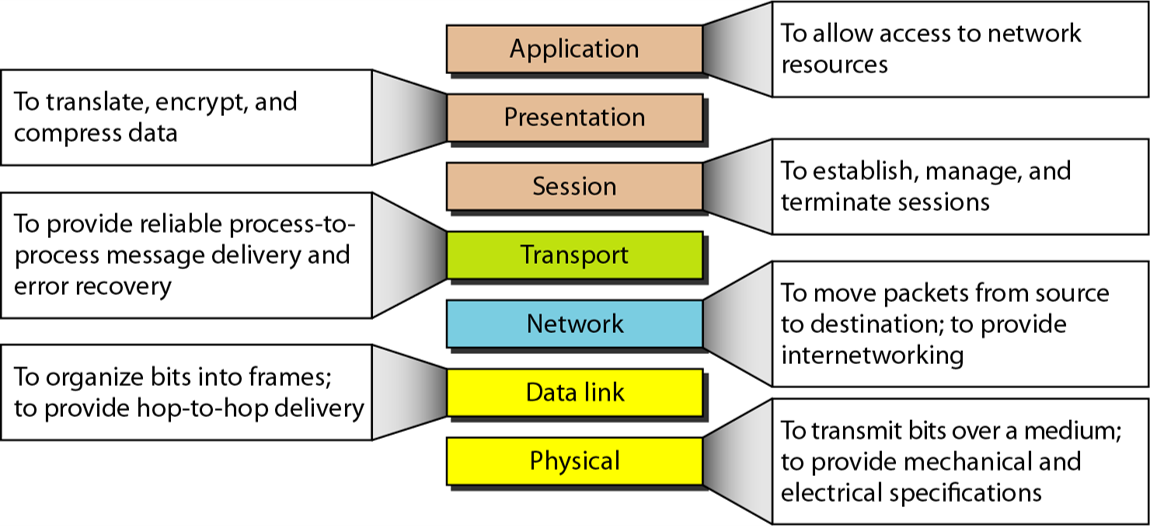
\includegraphics[width=0.9\columnwidth]{bab6/Picture15}
  \caption{Interleaving}
  \label{fig6:14}
\end{figure}

\begin{example}
  Four channels are multiplexed using TDM. If each channel sends 100 bytesis and we multiplex 1 byte per channel, show the frame traveling on the link, the size of the frame, the duration of a frame, the frame rate, and the bit rate for the link.
  \label{example6:8}
\end{example}

\begin{solution}
  The multiplexer is shown in Figure~\ref{fig6:15}. Each frame carries 1 byte from each channel; the size of each frame, therefore, is 4 bytes, or 32 bits. Because each channel is sending 100 bytes/s and a frame carries 1 byte from each channel, the frame rate must be 100 frames per second. The duration of a frame is therefore 11100 s. The link is carrying 100 frames per second, and since each frame contains 32 bits, the bit rate is 100 x 32, or 3200 bps. This is actually 4 times the bit rate of each channel, which is 100 x 8 =800 bps
\end{solution}

\begin{figure}[htbp]
  \centering
  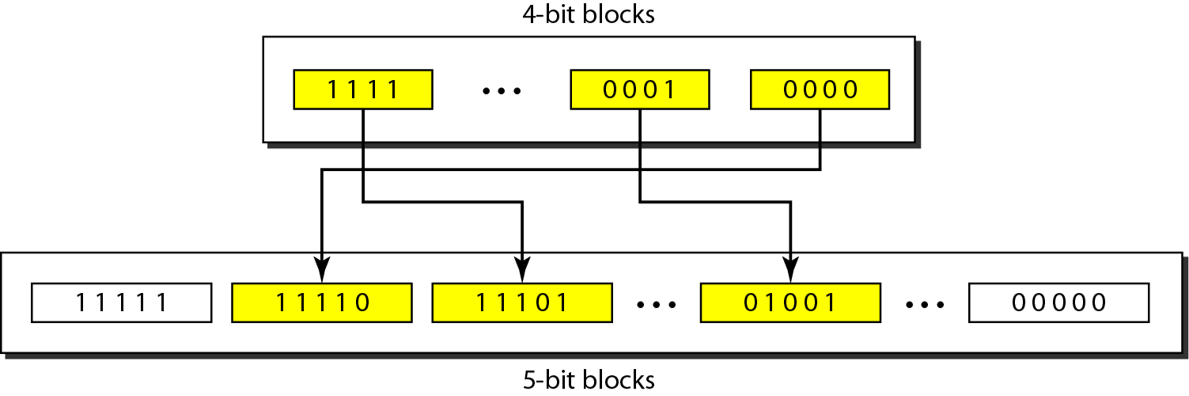
\includegraphics[width=0.9\columnwidth]{bab6/Picture16}
  \caption{Ilustrasi untuk contoh~\ref{example6:8}}
  \label{fig6:15}
\end{figure}

\begin{example}
  A multiplexer combines four 100-kbps channels using a time slot of 2 bits. Show the output with four arbitrary inputs. What is the frame rate? What is the frame duration? What is the bit rate? What is the bit duration?
  \label{example6:9}
\end{example}

\begin{solution}
  Figure~\ref{fig6:16} shows the output for four arbitrary inputs. The link carries 50,000 frames per second since each frame contains 2 bits per channel. The frame duration is therefore 1/50,000 s or 20 ~s. The frame rate is 50,000 frames per second, and each frame carries 8 bits; the bit rate is 50,000 x 8 =400,000 bits or 400 kbps. The bit duration is 1/400,000 s, or 2.5 IJ.s. Note that the frame duration is 8 times the bit duration because each frame is carrying 8 bits
\end{solution}

\begin{figure}[htbp]
  \centering
  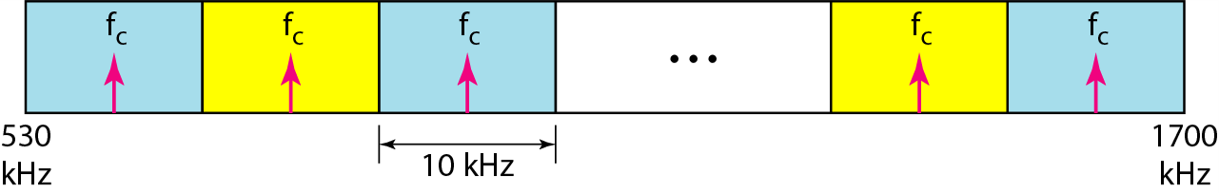
\includegraphics[width=0.9\columnwidth]{bab6/Picture17}
  \caption{Ilustrasi untuk contoh~\ref{example6:9}}
  \label{fig6:16}
\end{figure}

\subsection*{Empty Slots}
Synchronous TDM is not as efficient as it could be. If a source does not have data to send, the corresponding slot in the output frame is empty. Figure~\ref{fig6:17} shows a case in which one of the input lines has no data to send and one slot in another input line has discontinuous data.

\begin{figure}[htbp]
  \centering
  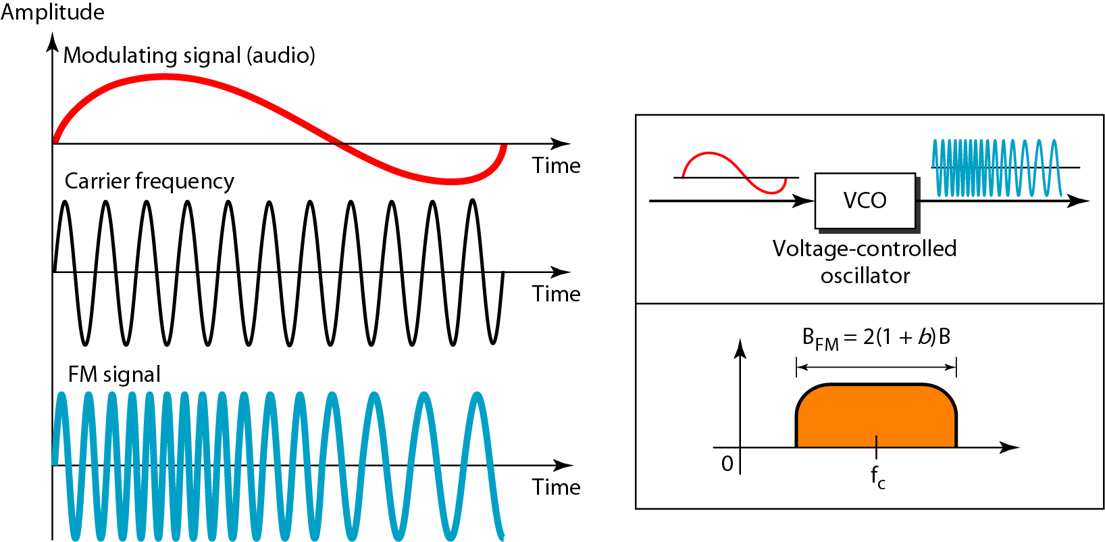
\includegraphics[width=0.9\columnwidth]{bab6/Picture18}
  \caption{Empty Slots}
  \label{fig6:17}
\end{figure}

The first output frame has three slots filled, the second frame has two slots filled, and the third frame has three slots filled. No frame is full. We learn in the next section that statistical TDM can improve the efficiency by removing the empty slots from the frame.

\subsubsection*{Data Rate Management}
One problem with TDM is how to handle a disparity in the input data rates. In all our discussion so far, we assumed that the data rates of all input lines were the same. However, if data rates are not the same, three strategies, or a combination of them, can be used. We call these three strategies multilevel multiplexing, multiple-slot allocation, and pulse stuffing.

\textbf{Multilevel Multiplexing} Multilevel multiplexing is a technique used when the data rate of an input line is a multiple of others. For example, in Figure~\ref{fig6:18}, we have two inputs of 20 kbps and three inputs of 40 kbps. The first two input lines can be multiplexed together to provide a data rate equal to the last three. A second level of multiplexing can create an output of 160 kbps.

\begin{figure}[htbp]
  \centering
  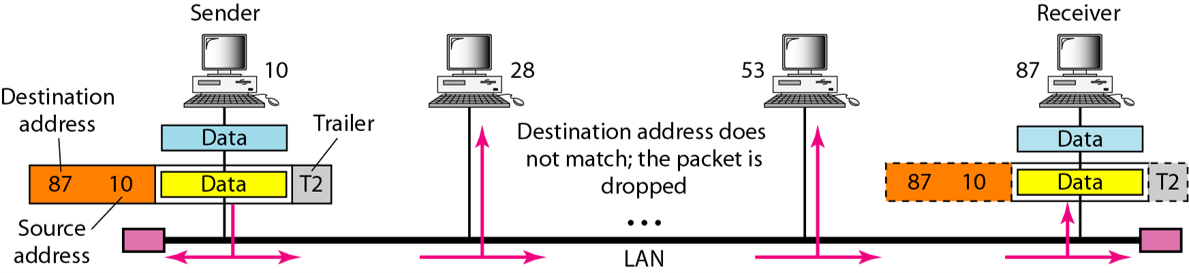
\includegraphics[width=0.9\columnwidth]{bab6/Picture19}
  \caption{Multilevel multiplexing}
  \label{fig6:18}
\end{figure}

\textbf{Multiple-Slot Allocation} Sometimes it is more efficient to allot more than one slot in a frame to a single input line. For example, we might have an input line that has a data rate that is a multiple of another input. In Figure~\ref{fig6:19}, the input line with a SO-kbps data rate can be given two slots in the output. We insert a serial-to-parallel converter in the line to make two inputs out of one.

\begin{figure}[htbp]
  \centering
  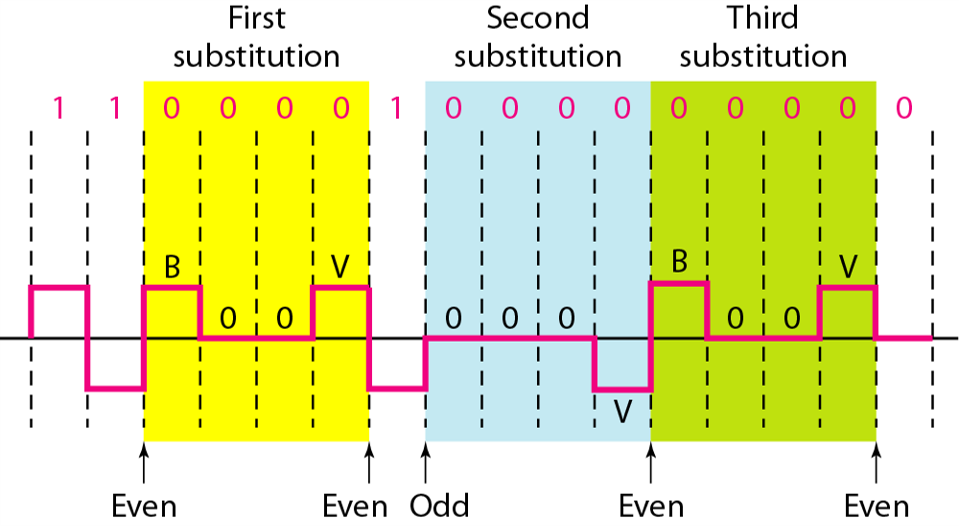
\includegraphics[width=0.9\columnwidth]{bab6/Picture20}
  \caption{Multiple-Slot allocation}
  \label{fig6:19}
\end{figure}

\textbf{Pulse Stuffing} Sometimes the bit rates of sources are not multiple integers of each other. Therefore, neither of the above two techniques can be applied. One solution is to make the highest input data rate the dominant data rate and then add dummy bits to the input lines with lower rates. This will increase their rates. This technique is called pulse stuffing, bit padding, or bit stuffing. The idea is shown in Figure~\ref{fig6:20}. The input with a data rate of 46 is pulse-stuffed to increase the rate to 50 kbps. Now multiplexing can take place.

\begin{figure}[htbp]
  \centering
  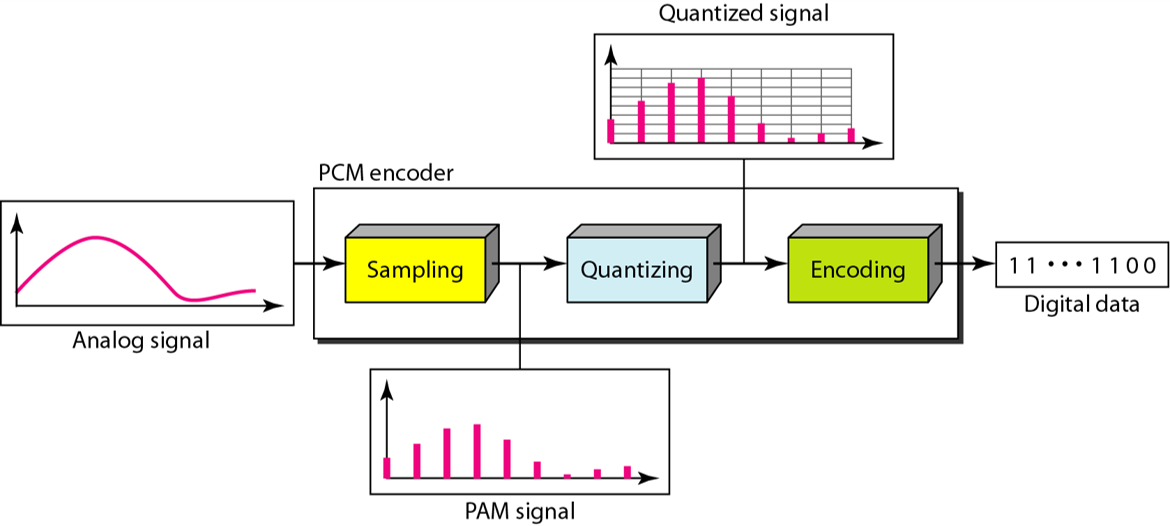
\includegraphics[width=0.9\columnwidth]{bab6/Picture21}
  \caption{Pulse stuffing}
  \label{fig6:20}
\end{figure}

\subsection*{Frame Synchronizing}
The implementation of TDM is not as simple as that of FDM. Synchronization between the multiplexer and demultiplexer is a major issue. If the. multiplexer and the demultiplexer are not synchronized, a bit belonging to one channel may be received by the wrong channel. For this reason, one or more synchronization bits are usually added to the beginning of each frame. These bits, called framing bits, follow a pattern, frame to frame, that allows the demultiplexer to synchronize with the incoming stream so that it can separate the time slots accurately. In most cases, this synchronization information consists of 1 bit per frame, alternating between 0 and I, as shown in Figure~\ref{fig6:21}.

\begin{figure}[htbp]
  \centering
  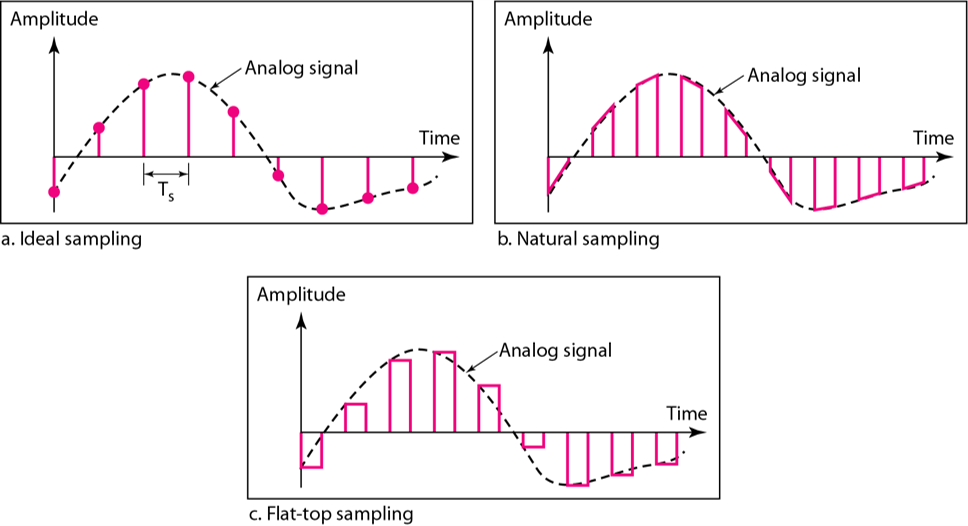
\includegraphics[width=0.9\columnwidth]{bab6/Picture22}
  \caption{Framing bits}
  \label{fig6:21}
\end{figure}

\begin{example}
  We have four sources, each creating 250 characters per second. If the interleaved unit is a character and 1 synchronizing bit is added to each frame, find (a) the data rate of each source, (b) the duration of each character in each source, (c) the frame rate, (d) the duration of each frame, (e) the number of bits in each frame, and (f) the data rate of the link.
  \label{example6:10}
\end{example}

\begin{solution}
  We can answer the questions as follows: 
  \begin{itemize}
    \item[a.] The data rate of each source is 250 $\times$ 8 = 2000 bps = 2 kbps.
    \item[b.] Each source sends 250 characters per second; therefore, the duration of a character is 1/250 s, or4 ms.
    \item[c.] Each frame has one character from each source, which means the link needs to send 250 frames per second to keep the transmission rate of each source.
    \item[d.] Theduration of each frame is 11250 s, or 4 ms. Note that the duration of each frame is the same as the duration of each character coming from each source.
    \item[e.] Each frame carries 4 characters and I extra synchronizing bit. This means that each frame is 4 $\times$ 8 + 1 = 33 bits.
    \item[f.] The link sends 250 frames per second, and each frame contains 33 bits. This means that the data rate of the link is 250 $\times$ 33, or 8250 bps. Note that the bit rate of the link is greater than the combined bit rates of the four channels. If we add the bit rates of four channels, we get 8000 bps. Because 250 frames are traveling per second and each contains 1 extra bit for synchronizing, we need to add 250 to the sum to get 8250 bps.
  \end{itemize}
\end{solution}

\vspace{12pt}

\begin{example}
  Two channels, one with a bit rate of 100 kbps and another with a bit rate of 200 kbps, are to be multiplexed. How this can be achieved? What is the frame rate? What is the frame duration? What is the bit rate of the link?
  \label{example6:11}
\end{example}

\begin{solution}
  We can allocate one slot to the first channel and two slots to the second channel. Each frame carries 3 bits. The frame rate is 100,000 frames per second because it carries 1 bit from the first channel. The frame duration is 1/100,000 s, or 10 ms. The bit rate is 100,000 frames/s x 3 bits per frame, or 300 kbps. Note that because each frame carries 1 bit from the first channel, the bit rate for the first channel is preserved. The bit rate for the second channel is also preserved because each frame carries 2 bits from the second channel.
\end{solution}

\subsection*{Digital Signal Service}
Telephone companies implement TDM through a hierarchy of digital signals, called digital signal (DS) service or digital hierarchy. Figure~\ref{fig6:22} shows the data rates supported by each level

\begin{figure}[htbp]
  \centering
  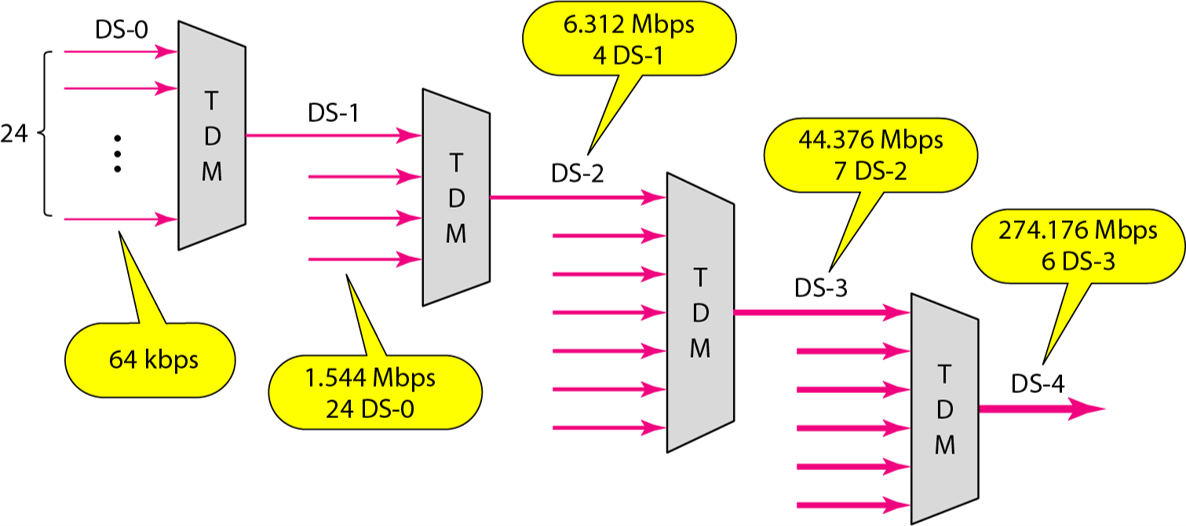
\includegraphics[width=0.9\columnwidth]{bab6/Picture23}
  \caption{Digital hierarchy}
  \label{fig6:22}
\end{figure}

\begin{itemize}
  \item[$\bullet$] A DS-0 service is a single digital channel of 64 kbps.
  \item[$\bullet$] DS-1 is a 1.544-Mbps service; 1.544 Mbps is 24 times 64 kbps plus 8 kbps of overhead. It can be used as a single service ons, or it can be used to multiplex 24 DS-O channels or to carry any other combination desired by the user that can fit within its 1.544-Mbps capacity.
  \item[$\bullet$] DS-3 is a 44.376-Mbps service; 44.376 Mbps is 672 times 64 kbps plus 1.368 Mbps of overhead. It can be used as a single service for 44.376-Mbps transmissions; or it can be used to multiplex 7 DS-2 channels, 28 DS-l channels, 672 DS-O channels, or a combination of these service types.
  \item[$\bullet$] DS-4 is a 274. 176-Mbps service; 274.176 is 4032 times 64 kbps plus 16.128 Mbps of overhead. It can be used to multiplex 6 DS-3 channels, 42 DS-2 channels, 168 DS-l channels, 4032 DS-O channels, or a combination ofthese service types
\end{itemize}

\subsection*{T Lines}
DS-0, DS-1, and so on are the names of services. To implement those services, the telephone companies use T lines (T-1 to T-4). These are lines with capacities precisely matched to the data rates of the DS-1 to DS-4 services (see Table 6.1). So far only T-1 and T-3 lines are commercially available.

\begin{table}[htbp]
  \centering
  \caption{DS and T line rates}
  \begin{tabular}{p{0.15\textwidth} p{0.15\textwidth} p{0.15\textwidth} p{0.15\textwidth}} 
   \toprule
   Sen/ice & Line & Rate (Mbps) & Voice Channels \\
   \midrule
   DS-1 & T-1 & 1.544 & 24 \\ 
   DS-2 & T-2 & 6.312 & 96 \\
   DS-3 & T-3 & 44.763 & 672 \\
   DS-4 & T-4 & 274.176 & 4032 \\
   \bottomrule
  \end{tabular}
  \label{tab6:1}
\end{table}

The T-1 line is used to implement DS-1; T-2 is used to implement DS-2; and so on. As you can see from Table~\ref{tab6:1}, DS-0 is not actually offered as a service, but it has been defined as a basis for reference purposes

\subsection*{T Lines for Analog Transmission}
T lines are digital lines designed for the transmission of digital data, audio, or video. However, they also can be used for analog transmission (regular telephone connections), provided the analog signals are first sampled, then time-division multiplexed.

The possibility of using T lines as analog carriers opened up a new generation of services for the telephone companies. Earlier, when an organization wanted 24 separate telephone lines, it needed to run 24 twisted-pair cables from the company to the central exchange. (Remember those old movies showing a busy executive with 10 telephones lined up on his desk? Or the old office telephones with a big fat cable running from them? Those cables contained a bundle of separate lines.) Today, that same organization can combine the 24 lines into one T-l line and run only the T-l line to the exchange. Figure~\ref{fig6:23} shows how 24 voice channels can be multiplexed onto one T-I line.

\begin{figure}[htbp]
  \centering
  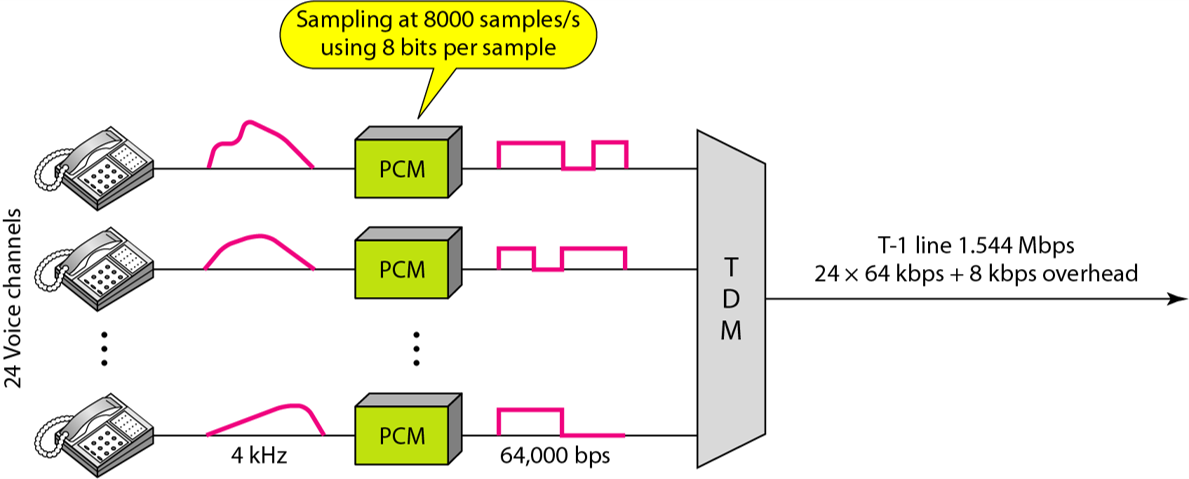
\includegraphics[width=0.9\columnwidth]{bab6/Picture24}
  \caption{T-1 line for multiplexing telephone lines}
  \label{fig6:23}
\end{figure}

The T-1 Frame As noted above, DS-1 requires 8 kbps of overhead. To understand how this overhead is calculated, we must examine the format of a 24-voice-channel frame. The frame used on a T-l line is usually 193 bits divided into 24 slots of 8 bits each plus 1 extra bit for synchronization (24 x 8 + 1 = 193); see Figure~\ref{fig6:24}. In other words, each slot contains one signal segment from each channel; 24 segments are interleaved in one frame. If a T-l line carries 8000 frames, the data rate is 1.544 Mbps (193 $\times$ 8000 = 1.544 Mbps)-the capacity of the line. Table 6.2 shows the E lines and their capacities.

\begin{figure}[htbp]
  \centering
  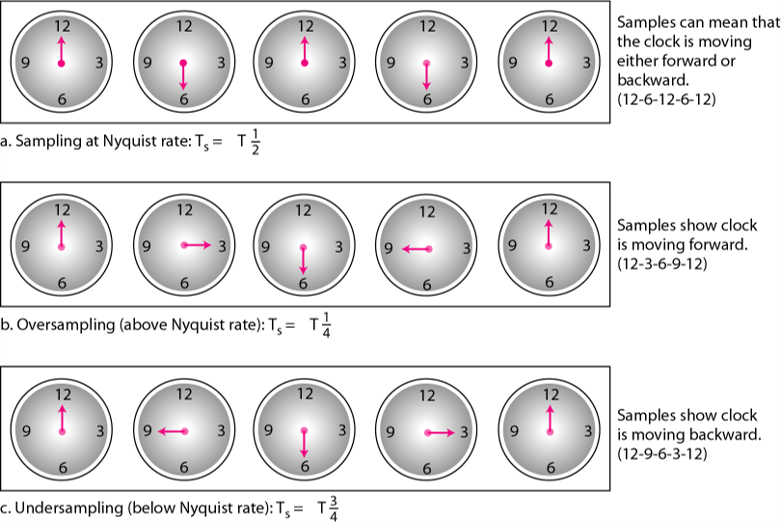
\includegraphics[width=0.9\columnwidth]{bab6/Picture25}
  \caption{T-1 frame structure}
  \label{fig6:24}
\end{figure}

\subsection*{E Lines}
Europeans use a version ofT lines called E lines. The two systems are conceptually identical, but their capacities differ. Table 6.2 shows the E lines and their capacities.

\begin{table}[htbp]
  \centering
  \caption{E line rates}
  \begin{tabular}{p{0.15\textwidth} p{0.15\textwidth} p{0.15\textwidth}} 
   \toprule
   Line & Rate (Mbps) & Voice Channels \\
   \midrule
   E-1 & 2.048 & 30 \\ 
   E-2 & 84.48 & 120 \\
   E-3 & 34.368 & 480 \\
   E-4 & 139.264 & 1920 \\
   \bottomrule
  \end{tabular}
  \label{tab6:2}
\end{table}

\subsection*{More Synchronous TDM Applications}
Some second-generation cellular telephone companies use synchronous TDM. For example, the digital version of cellular telephony divides the available bandwidth into 3D-kHz bands. For each band, TDM is applied so that six users can share the band. This means that each 3D-kHz band is now made of six time slots, and the digitized voice signals of the users are inserted in the slots. Using TDM, the number of telephone users in each area is now 6 times greater.

\subsection{Statistical Time-Division Multiplexing}
As we saw in the previous section, in synchronous TDM, each input has a reserved slot in the output frame. This can be inefficient if some input lines have no data to send. In statistical time-division multiplexing, slots are dynamically allocated to improve bandwidth efficiency. Only when an input line has a slot's worth of data to send is it given a slot in the output frame. In statistical multiplexing, the number of slots in each frame is less than the number of input lines. The multiplexer checks each input line in roundrobin fashion; it allocates a slot for an input line if the line has data to send; otherwise, it skips the line and checks the next line.

Figure~\ref{fig6:25} shows a synchronous and a statistical TDM example. In the former, some slots are empty because the corresponding line does not have data to send. In the latter, however, no slot is left empty as long as there are data to be sent by any input line.

\begin{figure}[htbp]
  \centering
  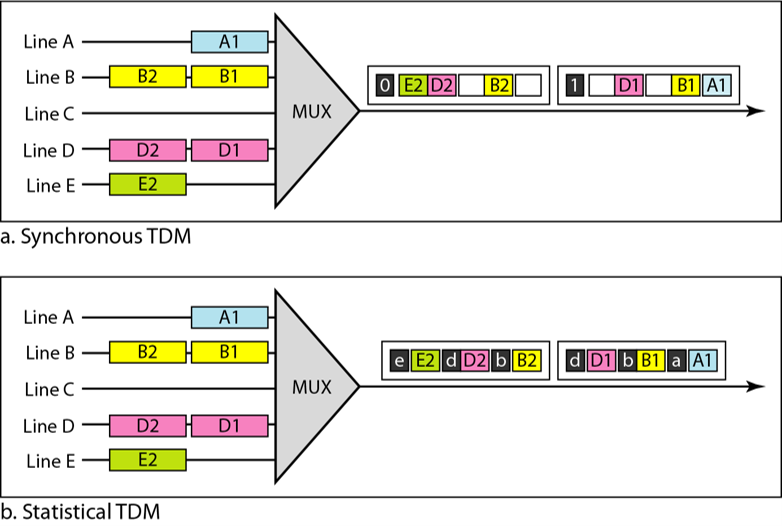
\includegraphics[width=0.9\columnwidth]{bab6/Picture26}
  \caption{TDM slot comparison}
  \label{fig6:25}
\end{figure}

\subsection*{Addressing}
Figure 6.26 also shows a major difference between slots in synchronous TDM and statistical TDM. An output slot in synchronous TDM is totally occupied by data; in statistical TDM, a slot needs to carry data as well as the address of the destination. In synchronous TDM, there is no need for addressing; synchronization and preassigned relationships between the inputs and outputs serve as an address. We know, for example, that input 1 always goes to input 2. If the multiplexer and the demultiplexer are synchronized, this is guaranteed. In statistical multiplexing, there is no fixed relationship between the inputs and outputs because there are no preassigned or reserved slots. We need to include the address of the receiver inside each slot to show where it is to be delivered. The addressing in its simplest form can be n bits to define N different output lines with n =10g2 N. For example, for eight different output lines, we need a 3-bit address.

\subsection*{Slot Size}
Since a slot carries both data and an address in statistical TDM, the ratio of the data size to address size must be reasonable to make transmission efficient. For example, it would be inefficient to send 1 bit per slot as data when the address is 3 bits. This would mean an overhead of 300 percent. In statistical TDM, a block of data is usually many bytes while the address is just a few bytes.

\subsection*{No Synchronization Bit}
There is another difference between synchronous and statistical TDM, but this time it is at the frame level. The frames in statistical TDM need not be synchronized, so we do not need synchronization bits.

\subsection*{Bandwidth}
In statistical TDM, the capacity of the link is normally less than the sum of the capacities of each channel. The designers of statistical TDM define the capacity of the link based on the statistics of the load for each channel. If on average only x percent of the input slots are filled, the capacity of the link reflects this. Of course, during peak times, some slots need to wait.


\section{Spread Spectrum}
Multiplexing combines signals from several sources to achieve bandwidth efficiency; the available bandwidth of a link is divided between the sources. In spread spectrum (88), we also combine signals from different sources to fit into a larger bandwidth, but our goals are somewhat different. Spread spectrum is designed to be used in wireless applications (LANs and WANs). In these types of applications, we have some concerns that outweigh bandwidth efficiency. In wireless applications, all stations use air (or a vacuum) as the medium for communication. Stations must be able to share this medium without interception by an eavesdropper and without being subject to jamming from a malicious intruder (in military operations, for example).

To achieve these goals, spread spectrum techniques add redundancy; they spread the original spectrum needed for each station. Ifthe required bandwidth for each station is B, spread spectrum expands it to Bss' such that Bss $\gg$ B. The expanded bandwidth allows the source to wrap its message in a protective envelope for a more secure transmission. An analogy is the sending of a delicate, expensive gift. We can insert the gift in a special box to prevent it from being damaged during transportation, and we can use a superior delivery service to guarantee the safety of the package.

\begin{figure}[htbp]
  \centering
  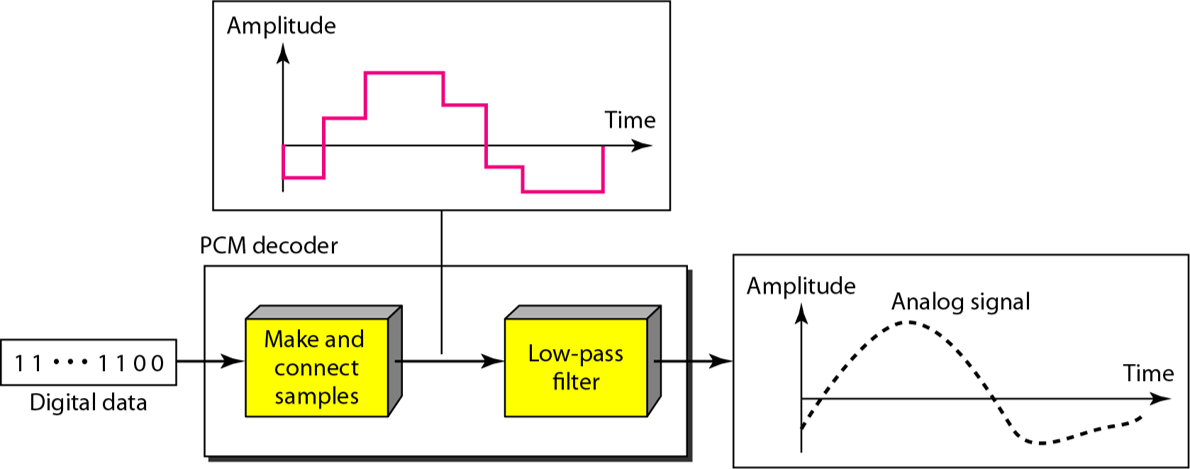
\includegraphics[width=0.9\columnwidth]{bab6/Picture27}
  \caption{Spread spectrum}
  \label{fig6:26}
\end{figure}

Figure 6.27 shows the idea of spread spectrum. Spread spectrum achieves its goals through two principles:
\begin{enumerate}
  \item The bandwidth allocated to each station needs to be, by far, larger than what is needed. This allows redundancy
  \item The expanding of the original bandwidth B to the bandwidth Bss must be done by a process that is independent of the original signal. In other words, the spreading process occurs after the signal is created by the source.
\end{enumerate}

After the signal is created by the source, the spreading process uses a spreading code and spreads the bandwidth. The figure shows the original bandwidth B and the spreaded bandwidth $B_{ss}$. The spreading code is a series of numbers that look random, but are actually a pattern.

There are two techniques to spread the bandwidth: frequency hopping spread spectrum (FHSS) and direct sequence spread spectrum (DSSS).


\subsection{Frequency Hopping Spread Spectrum (FHSS)}
The frequency hopping spread spectrum (FHSS) technique uses M different carrier frequencies that are modulated by the source signal. At one moment, the signal modulates one carrier frequency; at the next moment, the signal modulates another carrier frequency. Although the modulation is done using one carrier frequency at a time, M frequencies are used in the long run. The bandwidth occupied by a source after spreading is $B_{FHSS}$ $\gg$ B

Figure 6.28 shows the general layout for FHSS. A pseudorandom code generator, called pseudorandom noise (PN), creates a k-bit pattern for every hopping period $T_h$. The frequency table uses the pattern to find the frequency to be used for this hopping period and passes it to the frequency synthesizer. The frequency synthesizer creates a carrier signal of that frequency, and the source signal modulates the carrier signal

\begin{figure}[htbp]
  \centering
  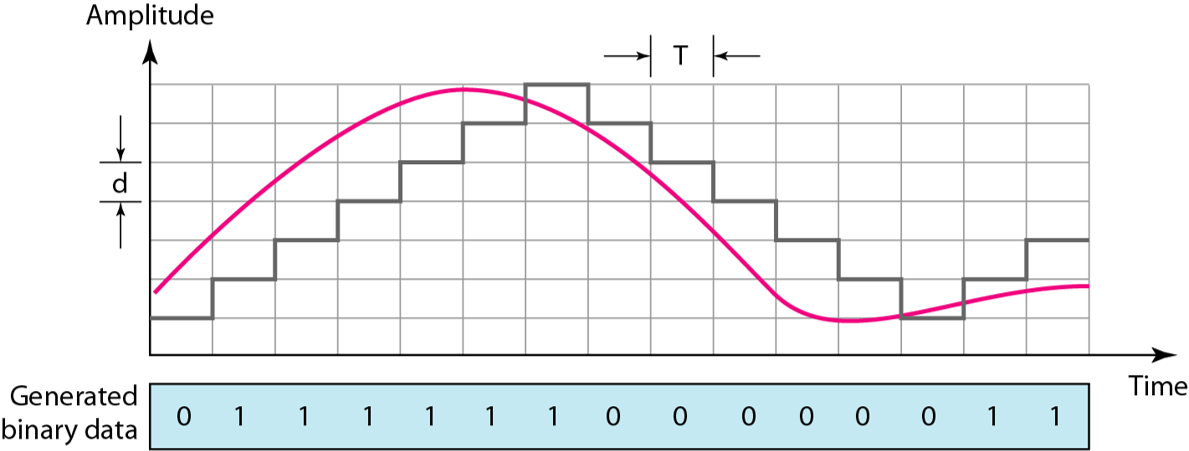
\includegraphics[width=0.9\columnwidth]{bab6/Picture28}
  \caption{Frequency hopping spread spectrum (FHSS)}
  \label{fig6:27}
\end{figure}

Suppose we have decided to have eight hopping frequencies. This is extremely low for real applications and isjust for illustration. In this case, Mis 8 and k is 3. The pseudorandom code generator will create eight different 3-bit patterns. These are mapped to eight different frequencies in the frequency table (see Figure 6.29).

\begin{figure}[htbp]
  \centering
  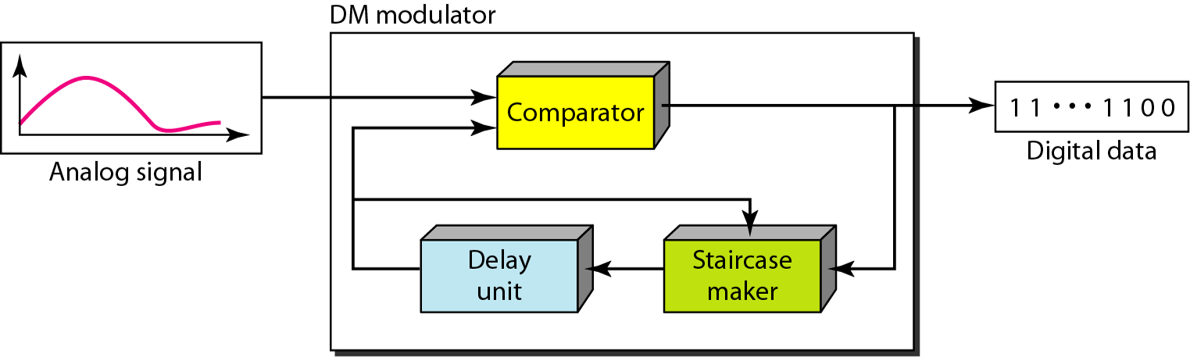
\includegraphics[width=0.9\columnwidth]{bab6/Picture29}
  \caption{Frequency selection in FHSS}
  \label{fig6:28}
\end{figure}

he pattern for this station is 101, 111, 001, 000, 010, all, 100. Note that the pattern is pseudorandom it is repeated after eight hoppings. This means that at hopping period 1, the pattern is 101. The frequency selected is 700 kHz; the source signal modulates this carrier frequency. The second k-bit pattern selected is 111, which selects the 900-kHz carrier; the eighth pattern is 100, the frequency is 600 kHz. After eight hoppings, the pattern repeats, starting from 101 again. Figure 6.30 shows how the signal hops around from carrier to carrier. We assume the required bandwidth of the original signal is 100 kHz.

\begin{figure}[htbp]
  \centering
  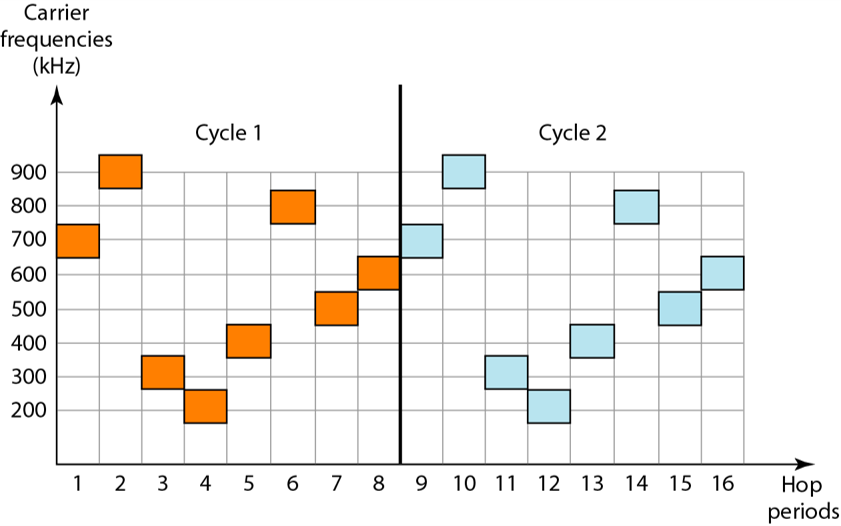
\includegraphics[width=0.9\columnwidth]{bab6/Picture30}
  \caption{FHSS cycles}
  \label{fig6:29}
\end{figure}

It can be shown that this scheme can accomplish the previously mentioned goals. If there are many k-bit patterns and the hopping period is short, a sender and receiver can have privacy. If an intruder tries to intercept the transmitted signal, she can only access a small piece of data because she does not know the spreading sequence to quickly adapt herself to the next hop. The scheme has also an antijamming effect. A malicious sender may be able to send noise to jam the signal for one hopping period (randomly), but not for the whole period.

\subsection*{Bandwidth Sharing}
If the number of hopping frequencies is M, we can multiplex M channels into one by using the same Bss bandwidth. This is possible because a station uses just one frequency in each hopping period; M - 1 other frequencies can be used by other M - 1 stations. In other words, M different stations can use the same Bss if an appropriate modulation technique such as multiple FSK (MFSK) is used. FHSS is similar to FDM, as shown in Figure 6.31.

Figure 6.31 shows an example of four channels using FDM and four channels using FHSS. In FDM, each station uses 11M of the bandwidth, but the allocation is fixed; in FHSS, each station uses 11M of the bandwidth, but the allocation changes hop to hop

\begin{figure}[htbp]
  \centering
  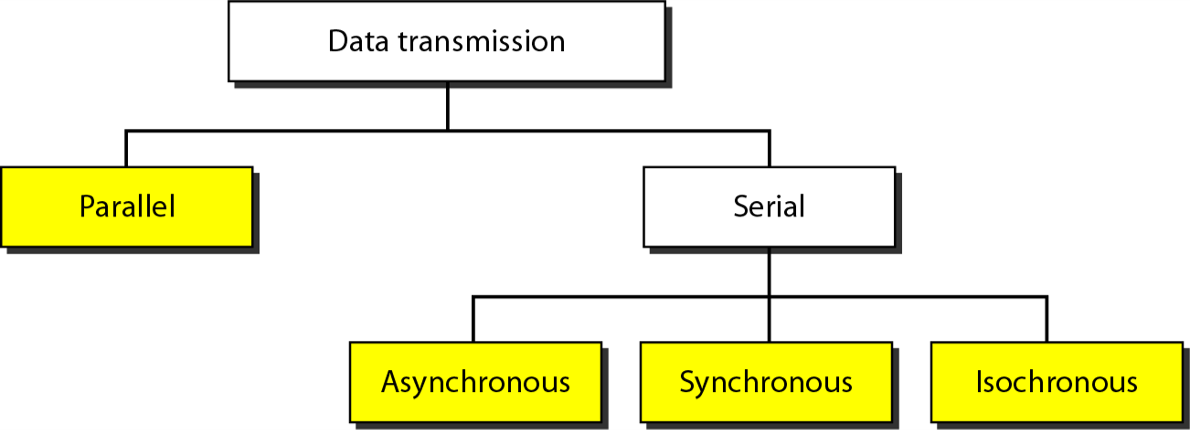
\includegraphics[width=0.9\columnwidth]{bab6/Picture31}
  \caption{Bandwidth sharing}
  \label{fig6:30}
\end{figure}

\subsection{Direct Sequence Spread Spectrum}
The direct sequence spread spectrum (DSSS) technique also expands the bandwidth of the original signal, but the process is different. In DSSS, we replace each data bit with 11 bits using a spreading code. In other words, each bit is assigned a code of 11 bits, called chips, where the chip rate is 11 times that of the data bit. Figure 6.32 shows the concept of DSSS.

\begin{figure}[htbp]
  \centering
  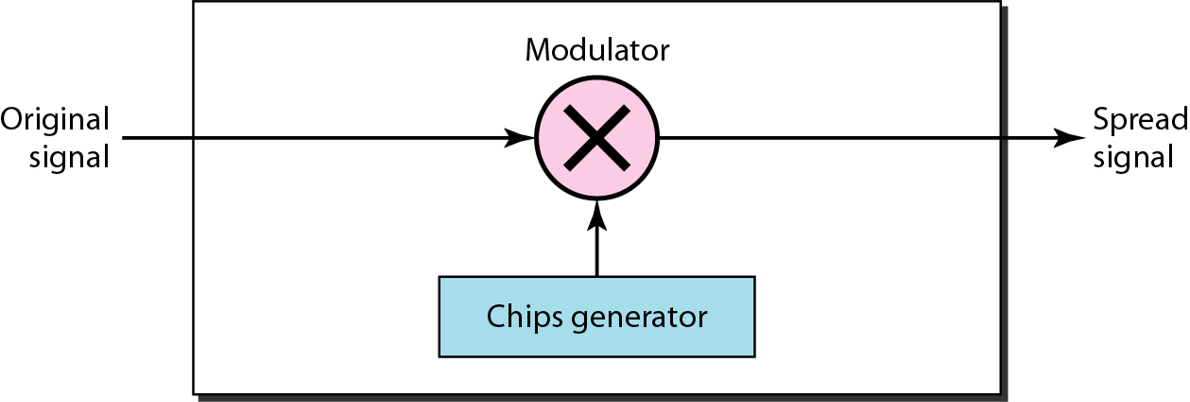
\includegraphics[width=0.9\columnwidth]{bab6/Picture32}
  \caption{Direct sequence spread spectrum}
  \label{fig6:31}
\end{figure}

As an example, let us consider the sequence used in a wireless LAN, the famous Barker sequence where 11 is 11. We assume that the original signal and the chips in the chip generator use polar NRZ encoding. Figure 6.33 shows the chips and the result of multiplying the original data by the chips to get the spread signal

In Figure 6.33, the spreading code is 11 chips having the pattern 10110111000 (in this case). If the original signal rate is N, the rate of the spread signal is lIN. This means that the required bandwidth for the spread signal is 11 times larger than the bandwidth of the original signal. The spread signal can provide privacy if the intruder does not know the code. It can also provide immunity against interference if each station uses a different code.

\begin{figure}[htbp]
  \centering
  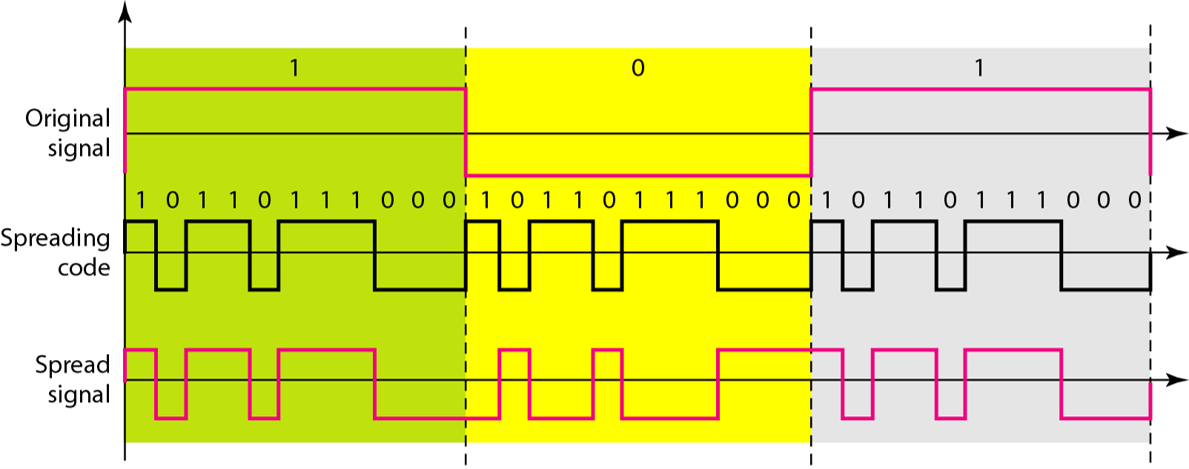
\includegraphics[width=0.9\columnwidth]{bab6/Picture33}
  \caption{DSSS example}
  \label{fig6:32}
\end{figure}

\subsection*{Bandwidth Sharing}
Can we share a bandwidth in DSSS as we did in FHSS? The answer is no and yes. If we use a spreading code that spreads signals (from different stations) that cannot be combined and separated, we cannot share a bandwidth. For example, as we will see in Chapter 14, some wireless LANs use DSSS and the spread bandwidth cannot be shared. However, if we use a special type of sequence code that allows the combining and separating of spread signals, we can share the bandwidth. As we will see in Chapter 16, a special spreading code allows us to use DSSS in cellular telephony and share a bandwidth between several users.

\section{Ringkasan}
\begin{itemize}
  \item[$\odot$] Bandwidth utilization is the use of available bandwidth to achieve specific goals. Efficiency can be achieved by using multiplexing; privacy and antijamming can be achieved by using spreading.
  \item[$\odot$] Multiplexing is the set of techniques that allows the simultaneous transmission of multiple signals across a single data link. In a multiplexed system, n lines share the bandwidth of one link. The word link refers to the physical path. The word channel refers to the portion of a link that carries a transmission.
  \item[$\odot$] There are three basic multiplexing techniques: frequency-division multiplexing, wavelength-division multiplexing, and time-division multiplexing. The first two are techniques designed for analog signals, the third, for digital signals
  \item[$\odot$] Frequency-division multiplexing (FDM) adalah teknik analog yang dapat diterapkan ketika bandwidth link (dalam hertz) lebih besar dari bandwidth gabungan dari sinyal yang akan ditransmisikan.
  \item[$\odot$] Wavelength-division multiplexing (WDM) is designed to use the high bandwidth capability of fiber-optic cable. WDM is an analog multiplexing technique to combine optical signals.
  \item[$\odot$] Time-division multiplexing (TDM) is a digital process that allows several connections to share the high bandwidth of a link. TDM is a digital multiplexing technique for combining several low-rate channels into one high-rate one
  \item[$\odot$] We can divide TDM into two different schemes: synchronous or statistical. In synchronous TDM, each input connection has an allotment in the output even if it is not sending data. In statistical TDM, slots are dynamically allocated to improve bandwidth efficiency
  \item[$\odot$] In spread spectrum (SS), we combine signals from different sources to fit into a larger bandwidth. Spread spectrum is designed to be used in wireless applications in which stations must be able to share the medium without interception by an eavesdropper and without being subject to jamming from a malicious intruder
  \item[$\odot$] The frequency hopping spread spectrum (FHSS) technique uses M different carrier frequencies that are modulated by the source signal. At one moment, the signal modulates one carrier frequency; at the next moment, the signal modulates another carrier frequency
  \item[$\odot$] The direct sequence spread spectrum (DSSS) technique expands the bandwidth of a signal by replacing each data bit with n bits using a spreading code. In other words, each bit is assigned a code of n bits, called chips.
\end{itemize}

\section{Latihan}

\subsection*{Pertanyaan ulasan}

\begin{enumerate}
  \item Describe the goals of multiplexing.
  \item List three main multiplexing techniques mentioned in this chapter. 
  \item Distinguish between a link and a channel in multiplexing. 
  \item Which of the three multiplexing techniques is (are) used to combine analog signals? Which ofthe three multiplexing techniques is (are) used to combine digital signals? 
  \item Define the analog hierarchy used by telephone companies and list different levels ofthe hierarchy. 
  \item Define the digital hierarchy used by telephone companies and list different levels of the hierarchy. 
  \item Which of the three multiplexing techniques is common for fiber optic links? Explain the reason. 
  \item Distinguish between multilevel TDM, multiple slot TDM, and pulse-stuffed TDM. 
  \item Distinguish between synchronous and statistical TDM. 
  \item Define spread spectrum and its goal. List the two spread spectrum techniques discussed in this chapter. 
  \item Define FHSS and explain how it achieves bandwidth spreading. 
  \item Define DSSS and explain how it achieves bandwidth spreading.
\end{enumerate}

\subsection*{Latihan}
\begin{enumerate}[resume]
  \item Assume that a voice channel occupies a bandwidth of 4 kHz. We need to multiplex 10 voice channels with guard bands of 500 Hz using FDM. Calculate the required bandwidth.
  \item We need to transmit 100 digitized voice channels using a pass-band channel of 20 KHz. What should be the ratio of bits/Hz if we use no guard band?
  \item In the analog hierarchy of Figure 6.9, find the overhead (extra bandwidth for guard band or control) in each hierarchy level (group, supergroup, master group, and jumbo group)
  \item We need to use synchronous TDM and combine 20 digital sources, each of 100 Kbps. Each output slot carries 1 bit from each digital source, but one extra bit is added to each frame for synchronization. Answer the following questions
  \item Repeat Exercise 16 if each output slot carries 2 bits from each source
  \item We have 14 sources, each creating 500 8-bit characters per second. Since only some of these sources are active at any moment, we use statistical TDM to combine these sources using character interleaving. Each frame carries 6 slots at a time, but we need to add four-bit addresses to each slot. Answer the following questions:
  \item Ten sources, six with a bit rate of 200 kbps and four with a bit rate of 400 kbps are to be combined using multilevel TDM with no synchronizing bits. Answer the following questions about the final stage of the multiplexing
  \item Four channels, two with a bit rate of 200 kbps and two with a bit rate of 150 kbps, are to be multiplexed using multiple slot TDM with no synchronization bits. Answer the following questions:
  \item Two channels, one with a bit rate of 190 kbps and another with a bit rate of 180 kbps, are to be multiplexed using pulse stuffing TDM with no synchronization bits. Answer the following questions:
  \item Answer the following questions about a T-1 line:
  \item Show the contents of the five output frames for a synchronous TDM multiplexer that combines four sources sending the following characters. Note that the characters are sent in the same order that they are typed. The third source is silent
  \item Figure 6.34 shows a multiplexer in a synchronous TDM system. Each output slot is only 10 bits long (3 bits taken from each input plus 1 framing bit). What is the output stream? The bits arrive at the multiplexer as shown by the arrows
  \item Figure 6.35 shows a demultiplexer in a synchronous TDM. If the input slot is 16 bits long (no framing bits), what is the bit stream in each output? The bits arrive at the demultiplexer as shown by the arrows
  \item Answer the following questions about the digital hierarchy in Figure 6.23
  \item What is the minimum number of bits in a PN sequence if we use FHSS with a channel bandwidth of B =4 KHz and Bss =100 KHz?
  \item An FHSS system uses a 4-bit PN sequence. If the bit rate of the PN is 64 bits per second, answer the following questions:
  \item A pseudorandom number generator uses the following formula to create a random series:
  \item We have a digital medium with a data rate of 10 Mbps. How many 64-kbps voice channels can be carried by this medium if we use DSSS with the Barker sequence?
\end{enumerate}
